
\documentclass{beamer}
\usepackage{setspace}
\usepackage{gensymb}
\usepackage{caption}
%\usepackage{multirow}
%\usepackage{multicolumn}
%\usepackage{subcaption}
%\doublespacing
\singlespacing
\usepackage{csvsimple}
\usepackage{amsmath}
\usepackage{multicol}
%\usepackage{enumerate}
\usepackage{amssymb}
%\usepackage{graphicx}
\usepackage{newfloat}
%\usepackage{syntax}
\usepackage{listings}
%\usepackage{iithtlc}
\usepackage{color}
\usepackage{tikz}
\usetikzlibrary{shapes,arrows}



%\usepackage{graphicx}
%\usepackage{amssymb}
%\usepackage{relsize}
%\usepackage[cmex10]{amsmath}
%\usepackage{mathtools}
%\usepackage{amsthm}
%\interdisplaylinepenalty=2500
%\savesymbol{iint}
%\usepackage{txfonts}
%\restoresymbol{TXF}{iint}
%\usepackage{wasysym}
\usepackage{amsthm}
\usepackage{mathrsfs}
\usepackage{txfonts}
\usepackage{stfloats}
\usepackage{cite}
\usepackage{cases}
\usepackage{mathtools}
\usepackage{caption}
\usepackage{enumerate}	
\usepackage{enumitem}
\usepackage{amsmath}
%\usepackage{xtab}
\usepackage{longtable}
\usepackage{multirow}
%\usepackage{algorithm}
%\usepackage{algpseudocode}
\usepackage{enumitem}
\usepackage{mathtools}
\usepackage{hyperref}
%\usepackage[framemethod=tikz]{mdframed}
\usepackage{listings}
    %\usepackage[latin1]{inputenc}                                 %%
    \usepackage{color}                                            %%
    \usepackage{array}                                            %%
    \usepackage{longtable}                                        %%
    \usepackage{calc}                                             %%
    \usepackage{multirow}                                         %%
    \usepackage{hhline}                                           %%
    \usepackage{ifthen}                                           %%
  %optionally (for landscape tables embedded in another document): %%
    \usepackage{lscape}     


\usepackage{url}
\def\UrlBreaks{\do\/\do-}


%\usepackage{stmaryrd}


%\usepackage{wasysym}
%\newcounter{MYtempeqncnt}
\DeclareMathOperator*{\Res}{Res}
%\renewcommand{\baselinestretch}{2}
\renewcommand\thesection{\arabic{section}}
\renewcommand\thesubsection{\thesection.\arabic{subsection}}
\renewcommand\thesubsubsection{\thesubsection.\arabic{subsubsection}}

%\renewcommand\thesectiondis{\arabic{section}}
%\renewcommand\thesubsectiondis{\thesectiondis.\arabic{subsection}}
%\renewcommand\thesubsubsectiondis{\thesubsectiondis.\arabic{subsubsection}}

% correct bad hyphenation here
\hyphenation{op-tical net-works semi-conduc-tor}

%\lstset{
%language=C,
%frame=single, 
%breaklines=true
%}

%\lstset{
	%%basicstyle=\small\ttfamily\bfseries,
	%%numberstyle=\small\ttfamily,
	%language=Octave,
	%backgroundcolor=\color{white},
	%%frame=single,
	%%keywordstyle=\bfseries,
	%%breaklines=true,
	%%showstringspaces=false,
	%%xleftmargin=-10mm,
	%%aboveskip=-1mm,
	%%belowskip=0mm
%}

%\surroundwithmdframed[width=\columnwidth]{lstlisting}
\def\inputGnumericTable{}                                 %%
\lstset{
%language=C,
frame=single, 
breaklines=true,
columns=fullflexible
}


\begin{document}
\title{\textbf{JEE matrix problem through Python}}   
\author{\textit{Raktim Gautam Goswami (EE17BTECH11051) \newline Abhishek Bairagi (EE17BTECH11004)}} 
\date{\today} 

\frame{\titlepage} 

\frame{\frametitle{Table of contents}\tableofcontents} 


\section{Problem Statement} 
\frame{\frametitle{Problem Statement} 
Find the locus of the point of intersection of
the lines: 
\[ \left( \begin{array}{cc}
\sqrt{2} & -1
\end{array} \right)
%
 \begin{matrix}
\textbf{x}
\end{matrix} 
\
%
 \begin{matrix}
+
\end{matrix} 
\
%
 \begin{matrix}
4\sqrt{2}k\
\end{matrix} 
\
%
 \begin{matrix}
 = 
\end{matrix} 
\
%
 \begin{matrix}
0
\end{matrix} 
\
\]

\[ \left( \begin{array}{cc}
\sqrt{2}k & k
\end{array} \right)
%
 \begin{matrix}
\textbf{x}
\end{matrix} 
\
%
 \begin{matrix}
-
\end{matrix} 
\
%
 \begin{matrix}
4\sqrt{2}\
\end{matrix} 
\
%
 \begin{matrix}
 = 
\end{matrix} 
\
%
 \begin{matrix}
0
\end{matrix} 
\
\]

}

\section{Figure 1}
\frame{\frametitle{Figure 1}
The figure for the above problem from plotting is as follows.
\begin{figure}
  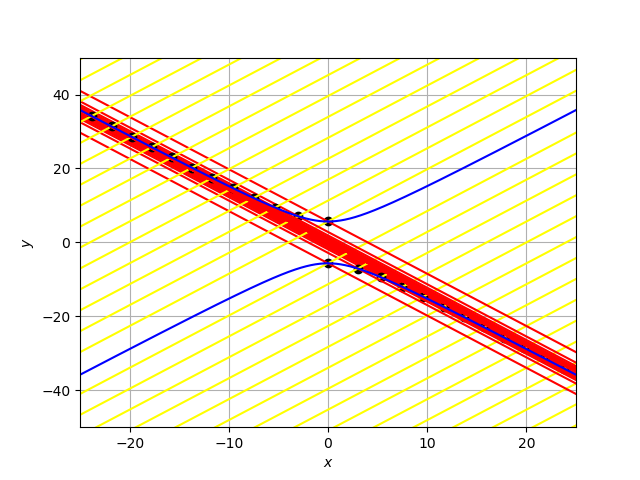
\includegraphics[width=200pt]{./Figs/Figure_1.png}
  
  \label{figure}
\end{figure}
}
\section{Figure 2}
\frame{\frametitle{Figure 2}
The family of first equation of lines.
\begin{figure}
  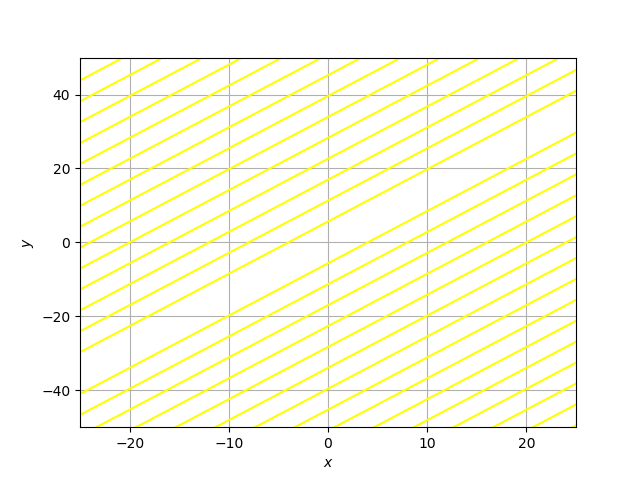
\includegraphics[width=200pt]{./Figs/Figure_2.png}
 
  \label{figure}
\end{figure}
}
\section{Figure 3}
\frame{\frametitle{Figure 3}
The family of second equation of lines.
\begin{figure}
  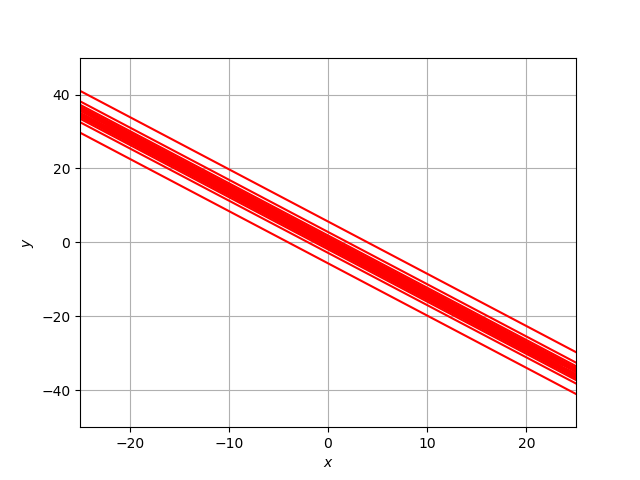
\includegraphics[width=200pt]{./Figs/Figure_3.png}
  
  \label{figure}
\end{figure}
}
\section{Figure 4}
\frame{\frametitle{Figure 4}
Their intersection points.
\begin{figure}
  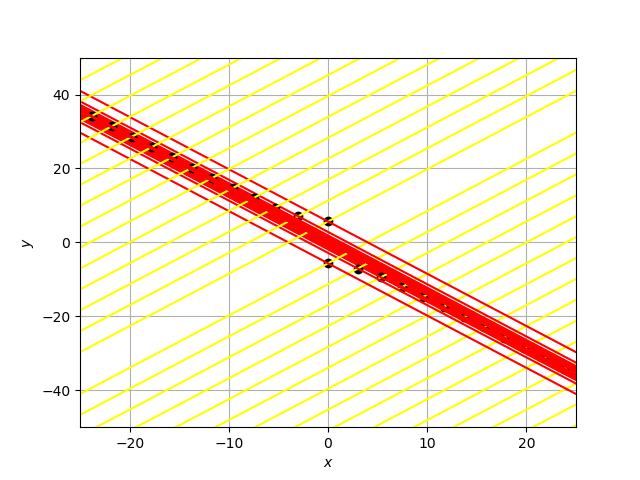
\includegraphics[width=200pt]{./Figs/Figure_4.png}
  
  \label{figure}
\end{figure}
}

\section{Figure 5}
\frame{\frametitle{Figure 5}
Final locus.
\begin{figure}
  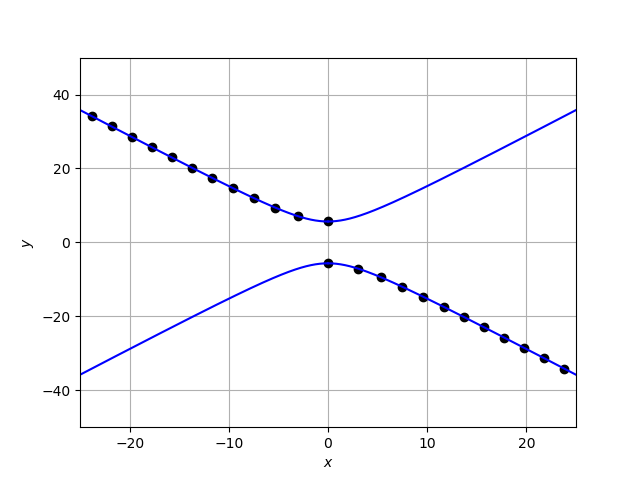
\includegraphics[width=200pt]{./Figs/Figure_5.png}
  
  \label{figure}
\end{figure}
}


\section{Steps to solve} 
\frame{\frametitle{Steps to solve}
\begin{itemize}
\item \textbf{Find value of k from first equation}\newline\newline
\item \textbf{Find transpose of k and use it in second equation.}\newline\newline
\item \textbf{Simplify the eqaution}\newline\newline
\item \textbf{Check the condition for conic.}\newline\newline
\end{itemize} 
}

\section{Solution}
\frame{\frametitle{Solution}
\begin{itemize}
\item \textbf{Find value of k from first equation}
\item \text{The given lines are:}\newline\newline
\[ \left( \begin{array}{cc}
\sqrt{2} & -1
\end{array} \right)
%
 \begin{matrix}
\textbf{x}
\end{matrix} 
\
%
 \begin{matrix}
+
\end{matrix} 
\
%
 \begin{matrix}
4\sqrt{2}k\
\end{matrix} 
\
%
 \begin{matrix}
 = 
\end{matrix} 
\
%
 \begin{matrix}
0
\end{matrix} 
\
\]

\[ \left( \begin{array}{cc}
\sqrt{2}k & k
\end{array} \right)
%
 \begin{matrix}
\textbf{x}
\end{matrix} 
\
%
 \begin{matrix}
-
\end{matrix} 
\
%
 \begin{matrix}
4\sqrt{2}\
\end{matrix} 
\
%
 \begin{matrix}
 = 
\end{matrix} 
\
%
 \begin{matrix}
0
\end{matrix} 
\
\]
\item \text{So from first line:}\newline\newline

\[  \begin{matrix}
k
\end{matrix} 
\
%
 \begin{matrix}
=
\end{matrix} 
\
%
%
 \begin{matrix}
-
\end{matrix} 
\
%
\left( \begin{array}{cc}
\sqrt{2} & -1
\end{array} \right)
%
 \begin{matrix}
x
\end{matrix} 
\
%
 \begin{matrix}
 /
\end{matrix} 
\
%
 \begin{matrix}
4\sqrt{2}
\end{matrix} 
\
\]


\end{itemize} 
}
\section{Solution ...}
So, 


\[\begin{matrix}
\textbf{$k^T$}
\end{matrix} 
\
%
\begin{matrix}
=
\end{matrix} 
\
%
\begin{matrix}
-
\end{matrix} 
\
%
\begin{matrix}
\textbf{$x^T$}
\end{matrix} 
\
%
\left( \begin{array}{cc}
\sqrt{2} \\
 -1
\end{array} \right)
% 
\begin{matrix}
 /
\end{matrix} 
\
%
 \begin{matrix}
4\sqrt{2}
\end{matrix} 
\
\]
And Second equation can be written as 

\[  \begin{matrix}
k
\end{matrix} 
\
%
\left( \begin{array}{cc}
\sqrt{2} & 1
\end{array} \right)
%
 \begin{matrix}
\textbf{x}
\end{matrix} 
\
%
 \begin{matrix}
=
\end{matrix} 
\
%
 \begin{matrix}
4\sqrt{2}\
\end{matrix} 
\
\]
Since k is a scalar, so

\[ \begin{matrix}
\textbf{$k^T =  k$}
\end{matrix} 
\
\]
So putting value of k in second equation we get:



\[
\begin{matrix}
\textbf{$x^T$}
\end{matrix} 
\
%
\left( \begin{array}{cc}
\sqrt{2} \\
 -1
\end{array} \right)
%
\left( \begin{array}{cc}
\sqrt{2} &1
\end{array} \right)
%
\begin{matrix}
\textbf{$x$}
\end{matrix} 
\
%
\begin{matrix}
=
\end{matrix} 
\
%
\begin{matrix}
-
\end{matrix} 
\
%
\begin{matrix}
\textbf{$32$}
\end{matrix} 
\
\]
\[
\begin{matrix}
\textbf{$x^T$}
\end{matrix} 
\
%
\left( \begin{array}{cc}
2 &\sqrt{2} \\
-\sqrt{2}& -1
\end{array} \right)
%
\begin{matrix}
\textbf{$x$}
\end{matrix} 
\
%
\begin{matrix}
+
\end{matrix} 
\
%
\begin{matrix}
\textbf{$32$}
\end{matrix} 
\
%
\begin{matrix}
=
\end{matrix} 
\
%
\begin{matrix}
0
\end{matrix} 
\
\]
This can be written as:

\[
\begin{matrix}
\textbf{$x^T$}
\end{matrix} 
\
%
\left( \begin{array}{cc}
2 &0 \\
0& -1
\end{array} \right)
%
\begin{matrix}
\textbf{$x$}
\end{matrix} 
\
%
\begin{matrix}
+
\end{matrix} 
\
\begin{matrix}
\textbf{$x^T$}
\end{matrix} 
\
%
\left( \begin{array}{cc}
0 &\sqrt{2} \\
-\sqrt{2}& 0
\end{array} \right)
%
\begin{matrix}
\textbf{$x$}
\end{matrix} 
\
%
\begin{matrix}
+
\end{matrix} 
\
%
\begin{matrix}
\textbf{$32$}
\end{matrix} 
\
%
\begin{matrix}
=
\end{matrix} 
\
%
\begin{matrix}
0
\end{matrix} 
\
\]
\section{Solution ...}
And
\[
\
\begin{matrix}
\textbf{$x^T$}
\end{matrix} 
\
%
\left( \begin{array}{cc}
0 &\sqrt{2} \\
-\sqrt{2}& 0
\end{array} \right)
%
\begin{matrix}
\textbf{$x$}
\end{matrix} 
\
%
\
\begin{matrix}
=
\end{matrix} 
\
%
\begin{matrix}
0
\end{matrix} 
\
\]
So
\[
\
\begin{matrix}
\textbf{$x^T$}
\end{matrix} 
\
%
\left( \begin{array}{cc}
2 &0 \\
0& -1
\end{array} \right)
%
\begin{matrix}
\textbf{$x$}
\end{matrix} 
\
%
\
\begin{matrix}
+
\end{matrix} 
\
%
\
\begin{matrix}
32
\end{matrix} 
\
%
\
\begin{matrix}
=
\end{matrix} 
\
%
\begin{matrix}
0
\end{matrix} 
\
\]
General equation of conic section:

\[
\
\begin{matrix}
\textbf{$x^T$}
\end{matrix} 
\
%
\
\begin{matrix}
V
\end{matrix} 
\
%
\begin{matrix}
\textbf{$x$}
\end{matrix} 
\
%
\
\begin{matrix}
+
\end{matrix} 
\
%
\
\begin{matrix}
2
\end{matrix} 
\
%
\
\begin{matrix}
\textbf{$u^T$}
\end{matrix} 
\
%
\begin{matrix}
x
\end{matrix} 
\
\begin{matrix}
+
\end{matrix} 
\
%
\
\begin{matrix}
F
\end{matrix} 
\
%
\
\begin{matrix}
=
\end{matrix} 
\
%
\begin{matrix}
0
\end{matrix} 
\
\]





\section{Conclusion} 
\frame{\frametitle{Final Conclusion}
\begin{itemize}
\item \text{On comparing our equation with general equation }\newline\newline
\item \text{We get det(V) as -2 which is less than 0.}\newline\newline
\item \text{So the conic is a hyperbola}\newline\newline
\item \text{So the locus of  the intersection point is a hyperbola.}\newline\newline
\end{itemize} 
}
\section{Code}
\frame{\frametitle{Code}
The link of the code can be found here -
\href{https://github.com/abhishekbairagi/EE1390-new/blob/master/Code/matrix3.py}{Matrix code}

}



\end{document}
